\documentclass[twoside]{book}

% Packages required by doxygen
\usepackage{calc}
\usepackage{doxygen}
\usepackage{graphicx}
\usepackage[utf8]{inputenc}
\usepackage{makeidx}
\usepackage{multicol}
\usepackage{multirow}
\usepackage{fixltx2e}
\PassOptionsToPackage{warn}{textcomp}
\usepackage{textcomp}
\usepackage[nointegrals]{wasysym}
\usepackage[table]{xcolor}

% Font selection
\usepackage[T1]{fontenc}
\usepackage{mathptmx}
\usepackage[scaled=.90]{helvet}
\usepackage{courier}
\usepackage{amssymb}
\usepackage{sectsty}
\renewcommand{\familydefault}{\sfdefault}
\allsectionsfont{%
  \fontseries{bc}\selectfont%
  \color{darkgray}%
}
\renewcommand{\DoxyLabelFont}{%
  \fontseries{bc}\selectfont%
  \color{darkgray}%
}
\newcommand{\+}{\discretionary{\mbox{\scriptsize$\hookleftarrow$}}{}{}}

% Page & text layout
\usepackage{geometry}
\geometry{%
  a4paper,%
  top=2.5cm,%
  bottom=2.5cm,%
  left=2.5cm,%
  right=2.5cm%
}
\tolerance=750
\hfuzz=15pt
\hbadness=750
\setlength{\emergencystretch}{15pt}
\setlength{\parindent}{0cm}
\setlength{\parskip}{0.2cm}
\makeatletter
\renewcommand{\paragraph}{%
  \@startsection{paragraph}{4}{0ex}{-1.0ex}{1.0ex}{%
    \normalfont\normalsize\bfseries\SS@parafont%
  }%
}
\renewcommand{\subparagraph}{%
  \@startsection{subparagraph}{5}{0ex}{-1.0ex}{1.0ex}{%
    \normalfont\normalsize\bfseries\SS@subparafont%
  }%
}
\makeatother

% Headers & footers
\usepackage{fancyhdr}
\pagestyle{fancyplain}
\fancyhead[LE]{\fancyplain{}{\bfseries\thepage}}
\fancyhead[CE]{\fancyplain{}{}}
\fancyhead[RE]{\fancyplain{}{\bfseries\leftmark}}
\fancyhead[LO]{\fancyplain{}{\bfseries\rightmark}}
\fancyhead[CO]{\fancyplain{}{}}
\fancyhead[RO]{\fancyplain{}{\bfseries\thepage}}
\fancyfoot[LE]{\fancyplain{}{}}
\fancyfoot[CE]{\fancyplain{}{}}
\fancyfoot[RE]{\fancyplain{}{\bfseries\scriptsize Generated on Wed Jul 30 2014 22\+:11\+:29 for Qualisys plugin for \char`\"{}\+Model Display\char`\"{} by Doxygen }}
\fancyfoot[LO]{\fancyplain{}{\bfseries\scriptsize Generated on Wed Jul 30 2014 22\+:11\+:29 for Qualisys plugin for \char`\"{}\+Model Display\char`\"{} by Doxygen }}
\fancyfoot[CO]{\fancyplain{}{}}
\fancyfoot[RO]{\fancyplain{}{}}
\renewcommand{\footrulewidth}{0.4pt}
\renewcommand{\chaptermark}[1]{%
  \markboth{#1}{}%
}
\renewcommand{\sectionmark}[1]{%
  \markright{\thesection\ #1}%
}

% Indices & bibliography
\usepackage{natbib}
\usepackage[titles]{tocloft}
\setcounter{tocdepth}{3}
\setcounter{secnumdepth}{5}
\makeindex

% Hyperlinks (required, but should be loaded last)
\usepackage{ifpdf}
\ifpdf
  \usepackage[pdftex,pagebackref=true]{hyperref}
\else
  \usepackage[ps2pdf,pagebackref=true]{hyperref}
\fi
\hypersetup{%
  colorlinks=true,%
  linkcolor=blue,%
  citecolor=blue,%
  unicode%
}

% Custom commands
\newcommand{\clearemptydoublepage}{%
  \newpage{\pagestyle{empty}\cleardoublepage}%
}


%===== C O N T E N T S =====

\begin{document}

% Titlepage & ToC
\hypersetup{pageanchor=false,
             bookmarks=true,
             bookmarksnumbered=true,
             pdfencoding=unicode
            }
\pagenumbering{roman}
\begin{titlepage}
\vspace*{7cm}
\begin{center}%
{\Large Qualisys plugin for \char`\"{}\+Model Display\char`\"{} \\[1ex]\large v1.\+0-\/0 }\\
\vspace*{1cm}
{\large Generated by Doxygen 1.8.7}\\
\vspace*{0.5cm}
{\small Wed Jul 30 2014 22:11:29}\\
\end{center}
\end{titlepage}
\clearemptydoublepage
\tableofcontents
\clearemptydoublepage
\pagenumbering{arabic}
\hypersetup{pageanchor=true}

%--- Begin generated contents ---
\chapter{Hierarchical Index}
\section{Class Hierarchy}
This inheritance list is sorted roughly, but not completely, alphabetically\+:\begin{DoxyCompactList}
\item Q\+Main\+Window\begin{DoxyCompactList}
\item \contentsline{section}{main\+Window}{\pageref{classmainWindow}}{}
\end{DoxyCompactList}
\item Q\+Widget\begin{DoxyCompactList}
\item \contentsline{section}{wind\+Data}{\pageref{classwindData}}{}
\end{DoxyCompactList}
\end{DoxyCompactList}

\chapter{Class Index}
\section{Class List}
Here are the classes, structs, unions and interfaces with brief descriptions\+:\begin{DoxyCompactList}
\item\contentsline{section}{\hyperlink{classmainWindow}{main\+Window} }{\pageref{classmainWindow}}{}
\item\contentsline{section}{\hyperlink{classwindData}{wind\+Data} }{\pageref{classwindData}}{}
\end{DoxyCompactList}

\chapter{File Index}
\section{File List}
Here is a list of all files with brief descriptions\+:\begin{DoxyCompactList}
\item\contentsline{section}{\hyperlink{sample_network_8cpp}{sample\+Network.\+cpp} }{\pageref{sample_network_8cpp}}{}
\item\contentsline{section}{\hyperlink{sample_network_8h}{sample\+Network.\+h} }{\pageref{sample_network_8h}}{}
\item\contentsline{section}{\hyperlink{sample_settings_8cpp}{sample\+Settings.\+cpp} }{\pageref{sample_settings_8cpp}}{}
\item\contentsline{section}{\hyperlink{sample_settings_8h}{sample\+Settings.\+h} }{\pageref{sample_settings_8h}}{}
\item\contentsline{section}{\hyperlink{wind_data_8cpp}{wind\+Data.\+cpp} }{\pageref{wind_data_8cpp}}{}
\item\contentsline{section}{\hyperlink{wind_data_8h}{wind\+Data.\+h} }{\pageref{wind_data_8h}}{}
\end{DoxyCompactList}

\chapter{Class Documentation}
\hypertarget{classsample_network}{\section{sample\+Network Class Reference}
\label{classsample_network}\index{sample\+Network@{sample\+Network}}
}


{\ttfamily \#include $<$sample\+Network.\+h$>$}



Inheritance diagram for sample\+Network\+:\nopagebreak
\begin{figure}[H]
\begin{center}
\leavevmode
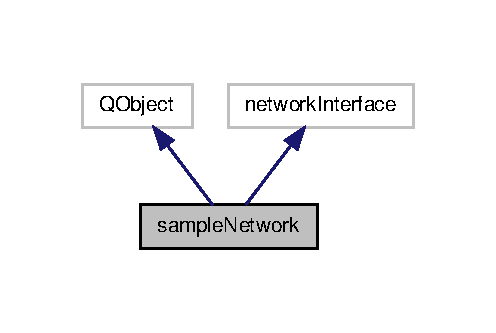
\includegraphics[width=238pt]{classsample_network__inherit__graph}
\end{center}
\end{figure}


Collaboration diagram for sample\+Network\+:\nopagebreak
\begin{figure}[H]
\begin{center}
\leavevmode
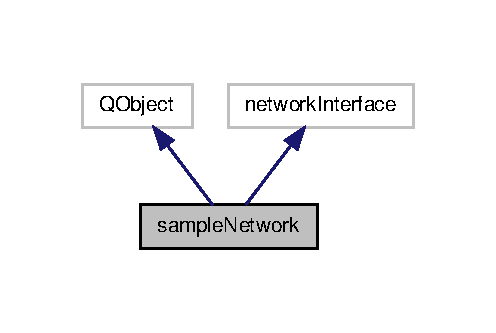
\includegraphics[width=238pt]{classsample_network__coll__graph}
\end{center}
\end{figure}
\subsection*{Public Slots}
\begin{DoxyCompactItemize}
\item 
virtual void \hyperlink{classsample_network_a5d7056c4114efdce6ea0e2c8f282f504}{connect\+To\+Peer} ()
\item 
virtual void \hyperlink{classsample_network_ac53b0506ff5dc44f3ab14ef8f5abe4d4}{disconnect\+From\+Peer} ()
\end{DoxyCompactItemize}
\subsection*{Signals}
\begin{DoxyCompactItemize}
\item 
void \hyperlink{classsample_network_ad19a0ebef5c19a91ca92e9c875f6cbfa}{plugin\+Running} ()
\end{DoxyCompactItemize}
\subsection*{Public Member Functions}
\begin{DoxyCompactItemize}
\item 
\hyperlink{classsample_network_ab1875223b2c14d15ff70309c02adec23}{sample\+Network} (Q\+Object $\ast$parent=0)
\item 
Q\+Object $\ast$ \hyperlink{classsample_network_aa8261b593056f9f81312f010c18e4e10}{as\+Q\+Object} ()
\item 
Q\+String \hyperlink{classsample_network_a6da8e8083bf841f351e98a3e0dbcbb50}{plugin\+Name} ()
\item 
Q\+String \hyperlink{classsample_network_a0ac04a041f0d2de3b56980f018005c49}{plugin\+Description} ()
\item 
Q\+String \hyperlink{classsample_network_ac5080eb5c66d260ae0be91e6624029c5}{xml\+Root\+Tag} ()
\item 
void \hyperlink{classsample_network_a775d11592b0e71db35a9c0907fa62d3e}{read\+X\+M\+L} (Q\+Dom\+Node root)
\item 
Q\+String\+List \hyperlink{classsample_network_a23a06ec2625e519f6835949db792e0a0}{write\+X\+M\+L} ()
\item 
Q\+Widget $\ast$ \hyperlink{classsample_network_af81ad6ecda7b0bb7be629cff9afbbd1b}{status\+Indicator} ()
\item 
Q\+Widget $\ast$ \hyperlink{classsample_network_af47008333333112350059d6e60fda18a}{settings\+Panel} ()
\item 
void \hyperlink{classsample_network_a897946986727579fe59ced0c10dce206}{store\+Settings} ()
\end{DoxyCompactItemize}


\subsection{Constructor \& Destructor Documentation}
\hypertarget{classsample_network_ab1875223b2c14d15ff70309c02adec23}{\index{sample\+Network@{sample\+Network}!sample\+Network@{sample\+Network}}
\index{sample\+Network@{sample\+Network}!sample\+Network@{sample\+Network}}
\subsubsection[{sample\+Network}]{\setlength{\rightskip}{0pt plus 5cm}sample\+Network\+::sample\+Network (
\begin{DoxyParamCaption}
\item[{Q\+Object $\ast$}]{parent = {\ttfamily 0}}
\end{DoxyParamCaption}
)}}\label{classsample_network_ab1875223b2c14d15ff70309c02adec23}


\subsection{Member Function Documentation}
\hypertarget{classsample_network_aa8261b593056f9f81312f010c18e4e10}{\index{sample\+Network@{sample\+Network}!as\+Q\+Object@{as\+Q\+Object}}
\index{as\+Q\+Object@{as\+Q\+Object}!sample\+Network@{sample\+Network}}
\subsubsection[{as\+Q\+Object}]{\setlength{\rightskip}{0pt plus 5cm}Q\+Object $\ast$ sample\+Network\+::as\+Q\+Object (
\begin{DoxyParamCaption}
{}
\end{DoxyParamCaption}
)}}\label{classsample_network_aa8261b593056f9f81312f010c18e4e10}
\hypertarget{classsample_network_a5d7056c4114efdce6ea0e2c8f282f504}{\index{sample\+Network@{sample\+Network}!connect\+To\+Peer@{connect\+To\+Peer}}
\index{connect\+To\+Peer@{connect\+To\+Peer}!sample\+Network@{sample\+Network}}
\subsubsection[{connect\+To\+Peer}]{\setlength{\rightskip}{0pt plus 5cm}void sample\+Network\+::connect\+To\+Peer (
\begin{DoxyParamCaption}
{}
\end{DoxyParamCaption}
)\hspace{0.3cm}{\ttfamily [virtual]}, {\ttfamily [slot]}}}\label{classsample_network_a5d7056c4114efdce6ea0e2c8f282f504}
\hypertarget{classsample_network_ac53b0506ff5dc44f3ab14ef8f5abe4d4}{\index{sample\+Network@{sample\+Network}!disconnect\+From\+Peer@{disconnect\+From\+Peer}}
\index{disconnect\+From\+Peer@{disconnect\+From\+Peer}!sample\+Network@{sample\+Network}}
\subsubsection[{disconnect\+From\+Peer}]{\setlength{\rightskip}{0pt plus 5cm}void sample\+Network\+::disconnect\+From\+Peer (
\begin{DoxyParamCaption}
{}
\end{DoxyParamCaption}
)\hspace{0.3cm}{\ttfamily [virtual]}, {\ttfamily [slot]}}}\label{classsample_network_ac53b0506ff5dc44f3ab14ef8f5abe4d4}
\hypertarget{classsample_network_a0ac04a041f0d2de3b56980f018005c49}{\index{sample\+Network@{sample\+Network}!plugin\+Description@{plugin\+Description}}
\index{plugin\+Description@{plugin\+Description}!sample\+Network@{sample\+Network}}
\subsubsection[{plugin\+Description}]{\setlength{\rightskip}{0pt plus 5cm}Q\+String sample\+Network\+::plugin\+Description (
\begin{DoxyParamCaption}
{}
\end{DoxyParamCaption}
)}}\label{classsample_network_a0ac04a041f0d2de3b56980f018005c49}
\hypertarget{classsample_network_a6da8e8083bf841f351e98a3e0dbcbb50}{\index{sample\+Network@{sample\+Network}!plugin\+Name@{plugin\+Name}}
\index{plugin\+Name@{plugin\+Name}!sample\+Network@{sample\+Network}}
\subsubsection[{plugin\+Name}]{\setlength{\rightskip}{0pt plus 5cm}Q\+String sample\+Network\+::plugin\+Name (
\begin{DoxyParamCaption}
{}
\end{DoxyParamCaption}
)}}\label{classsample_network_a6da8e8083bf841f351e98a3e0dbcbb50}
\hypertarget{classsample_network_ad19a0ebef5c19a91ca92e9c875f6cbfa}{\index{sample\+Network@{sample\+Network}!plugin\+Running@{plugin\+Running}}
\index{plugin\+Running@{plugin\+Running}!sample\+Network@{sample\+Network}}
\subsubsection[{plugin\+Running}]{\setlength{\rightskip}{0pt plus 5cm}void sample\+Network\+::plugin\+Running (
\begin{DoxyParamCaption}
{}
\end{DoxyParamCaption}
)\hspace{0.3cm}{\ttfamily [signal]}}}\label{classsample_network_ad19a0ebef5c19a91ca92e9c875f6cbfa}
\hypertarget{classsample_network_a775d11592b0e71db35a9c0907fa62d3e}{\index{sample\+Network@{sample\+Network}!read\+X\+M\+L@{read\+X\+M\+L}}
\index{read\+X\+M\+L@{read\+X\+M\+L}!sample\+Network@{sample\+Network}}
\subsubsection[{read\+X\+M\+L}]{\setlength{\rightskip}{0pt plus 5cm}void sample\+Network\+::read\+X\+M\+L (
\begin{DoxyParamCaption}
\item[{Q\+Dom\+Node}]{root}
\end{DoxyParamCaption}
)}}\label{classsample_network_a775d11592b0e71db35a9c0907fa62d3e}
\hypertarget{classsample_network_af47008333333112350059d6e60fda18a}{\index{sample\+Network@{sample\+Network}!settings\+Panel@{settings\+Panel}}
\index{settings\+Panel@{settings\+Panel}!sample\+Network@{sample\+Network}}
\subsubsection[{settings\+Panel}]{\setlength{\rightskip}{0pt plus 5cm}Q\+Widget $\ast$ sample\+Network\+::settings\+Panel (
\begin{DoxyParamCaption}
{}
\end{DoxyParamCaption}
)}}\label{classsample_network_af47008333333112350059d6e60fda18a}
\hypertarget{classsample_network_af81ad6ecda7b0bb7be629cff9afbbd1b}{\index{sample\+Network@{sample\+Network}!status\+Indicator@{status\+Indicator}}
\index{status\+Indicator@{status\+Indicator}!sample\+Network@{sample\+Network}}
\subsubsection[{status\+Indicator}]{\setlength{\rightskip}{0pt plus 5cm}Q\+Widget $\ast$ sample\+Network\+::status\+Indicator (
\begin{DoxyParamCaption}
{}
\end{DoxyParamCaption}
)}}\label{classsample_network_af81ad6ecda7b0bb7be629cff9afbbd1b}
\hypertarget{classsample_network_a897946986727579fe59ced0c10dce206}{\index{sample\+Network@{sample\+Network}!store\+Settings@{store\+Settings}}
\index{store\+Settings@{store\+Settings}!sample\+Network@{sample\+Network}}
\subsubsection[{store\+Settings}]{\setlength{\rightskip}{0pt plus 5cm}void sample\+Network\+::store\+Settings (
\begin{DoxyParamCaption}
{}
\end{DoxyParamCaption}
)}}\label{classsample_network_a897946986727579fe59ced0c10dce206}
\hypertarget{classsample_network_a23a06ec2625e519f6835949db792e0a0}{\index{sample\+Network@{sample\+Network}!write\+X\+M\+L@{write\+X\+M\+L}}
\index{write\+X\+M\+L@{write\+X\+M\+L}!sample\+Network@{sample\+Network}}
\subsubsection[{write\+X\+M\+L}]{\setlength{\rightskip}{0pt plus 5cm}Q\+String\+List sample\+Network\+::write\+X\+M\+L (
\begin{DoxyParamCaption}
{}
\end{DoxyParamCaption}
)}}\label{classsample_network_a23a06ec2625e519f6835949db792e0a0}
\hypertarget{classsample_network_ac5080eb5c66d260ae0be91e6624029c5}{\index{sample\+Network@{sample\+Network}!xml\+Root\+Tag@{xml\+Root\+Tag}}
\index{xml\+Root\+Tag@{xml\+Root\+Tag}!sample\+Network@{sample\+Network}}
\subsubsection[{xml\+Root\+Tag}]{\setlength{\rightskip}{0pt plus 5cm}Q\+String sample\+Network\+::xml\+Root\+Tag (
\begin{DoxyParamCaption}
{}
\end{DoxyParamCaption}
)}}\label{classsample_network_ac5080eb5c66d260ae0be91e6624029c5}


The documentation for this class was generated from the following files\+:\begin{DoxyCompactItemize}
\item 
\hyperlink{sample_network_8h}{sample\+Network.\+h}\item 
\hyperlink{sample_network_8cpp}{sample\+Network.\+cpp}\end{DoxyCompactItemize}

\hypertarget{classsample_settings}{\section{sample\+Settings Class Reference}
\label{classsample_settings}\index{sample\+Settings@{sample\+Settings}}
}


{\ttfamily \#include $<$sample\+Settings.\+h$>$}

\subsection*{Public Member Functions}
\begin{DoxyCompactItemize}
\item 
\hyperlink{classsample_settings_a3ae7a15cc1b8cf55d57139a0976f9dfd}{sample\+Settings} ()
\item 
void \hyperlink{classsample_settings_a2ab1eb40b65cddcad17c556f43fa2667}{read\+X\+M\+L} (Q\+Dom\+Node root)
\item 
Q\+String\+List \hyperlink{classsample_settings_a0996a76fb953ad9f5b7464cb328e60a4}{write\+X\+M\+L} ()
\item 
void \hyperlink{classsample_settings_ae87dbb0454d5dd59ba666fecf149cac7}{store\+G\+U\+I\+Values} ()
\end{DoxyCompactItemize}
\subsection*{Public Attributes}
\begin{DoxyCompactItemize}
\item 
Q\+String \hyperlink{classsample_settings_a1936cbf3ca632352dc75c1ecc30d9ec4}{host}
\item 
int \hyperlink{classsample_settings_a174a34a6ac173e8ded1b1496526a207e}{port}
\item 
int \hyperlink{classsample_settings_aa10ab5fff05664b7249873cea20c8164}{reconnect\+Rate}
\item 
int \hyperlink{classsample_settings_a4ea02c94b4f50acfefc8d9d8bea23868}{connect\+Timeout}
\item 
int \hyperlink{classsample_settings_a6fbeef484a848dc677b7e6d4f1526cbc}{message\+Timeout}
\item 
bool \hyperlink{classsample_settings_a4660e80373002545aa3ac363b47e709a}{auto\+Reconnect}
\item 
Q\+Widget $\ast$ \hyperlink{classsample_settings_a82b13a40ed430cce65c6e709858b792a}{gui\+Panel}
\end{DoxyCompactItemize}


\subsection{Constructor \& Destructor Documentation}
\hypertarget{classsample_settings_a3ae7a15cc1b8cf55d57139a0976f9dfd}{\index{sample\+Settings@{sample\+Settings}!sample\+Settings@{sample\+Settings}}
\index{sample\+Settings@{sample\+Settings}!sample\+Settings@{sample\+Settings}}
\subsubsection[{sample\+Settings}]{\setlength{\rightskip}{0pt plus 5cm}sample\+Settings\+::sample\+Settings (
\begin{DoxyParamCaption}
{}
\end{DoxyParamCaption}
)}}\label{classsample_settings_a3ae7a15cc1b8cf55d57139a0976f9dfd}


\subsection{Member Function Documentation}
\hypertarget{classsample_settings_a2ab1eb40b65cddcad17c556f43fa2667}{\index{sample\+Settings@{sample\+Settings}!read\+X\+M\+L@{read\+X\+M\+L}}
\index{read\+X\+M\+L@{read\+X\+M\+L}!sample\+Settings@{sample\+Settings}}
\subsubsection[{read\+X\+M\+L}]{\setlength{\rightskip}{0pt plus 5cm}void sample\+Settings\+::read\+X\+M\+L (
\begin{DoxyParamCaption}
\item[{Q\+Dom\+Node}]{root}
\end{DoxyParamCaption}
)}}\label{classsample_settings_a2ab1eb40b65cddcad17c556f43fa2667}
\hypertarget{classsample_settings_ae87dbb0454d5dd59ba666fecf149cac7}{\index{sample\+Settings@{sample\+Settings}!store\+G\+U\+I\+Values@{store\+G\+U\+I\+Values}}
\index{store\+G\+U\+I\+Values@{store\+G\+U\+I\+Values}!sample\+Settings@{sample\+Settings}}
\subsubsection[{store\+G\+U\+I\+Values}]{\setlength{\rightskip}{0pt plus 5cm}void sample\+Settings\+::store\+G\+U\+I\+Values (
\begin{DoxyParamCaption}
{}
\end{DoxyParamCaption}
)}}\label{classsample_settings_ae87dbb0454d5dd59ba666fecf149cac7}
\hypertarget{classsample_settings_a0996a76fb953ad9f5b7464cb328e60a4}{\index{sample\+Settings@{sample\+Settings}!write\+X\+M\+L@{write\+X\+M\+L}}
\index{write\+X\+M\+L@{write\+X\+M\+L}!sample\+Settings@{sample\+Settings}}
\subsubsection[{write\+X\+M\+L}]{\setlength{\rightskip}{0pt plus 5cm}Q\+String\+List sample\+Settings\+::write\+X\+M\+L (
\begin{DoxyParamCaption}
{}
\end{DoxyParamCaption}
)}}\label{classsample_settings_a0996a76fb953ad9f5b7464cb328e60a4}


\subsection{Member Data Documentation}
\hypertarget{classsample_settings_a4660e80373002545aa3ac363b47e709a}{\index{sample\+Settings@{sample\+Settings}!auto\+Reconnect@{auto\+Reconnect}}
\index{auto\+Reconnect@{auto\+Reconnect}!sample\+Settings@{sample\+Settings}}
\subsubsection[{auto\+Reconnect}]{\setlength{\rightskip}{0pt plus 5cm}bool sample\+Settings\+::auto\+Reconnect}}\label{classsample_settings_a4660e80373002545aa3ac363b47e709a}
\hypertarget{classsample_settings_a4ea02c94b4f50acfefc8d9d8bea23868}{\index{sample\+Settings@{sample\+Settings}!connect\+Timeout@{connect\+Timeout}}
\index{connect\+Timeout@{connect\+Timeout}!sample\+Settings@{sample\+Settings}}
\subsubsection[{connect\+Timeout}]{\setlength{\rightskip}{0pt plus 5cm}int sample\+Settings\+::connect\+Timeout}}\label{classsample_settings_a4ea02c94b4f50acfefc8d9d8bea23868}
\hypertarget{classsample_settings_a82b13a40ed430cce65c6e709858b792a}{\index{sample\+Settings@{sample\+Settings}!gui\+Panel@{gui\+Panel}}
\index{gui\+Panel@{gui\+Panel}!sample\+Settings@{sample\+Settings}}
\subsubsection[{gui\+Panel}]{\setlength{\rightskip}{0pt plus 5cm}Q\+Widget$\ast$ sample\+Settings\+::gui\+Panel}}\label{classsample_settings_a82b13a40ed430cce65c6e709858b792a}
\hypertarget{classsample_settings_a1936cbf3ca632352dc75c1ecc30d9ec4}{\index{sample\+Settings@{sample\+Settings}!host@{host}}
\index{host@{host}!sample\+Settings@{sample\+Settings}}
\subsubsection[{host}]{\setlength{\rightskip}{0pt plus 5cm}Q\+String sample\+Settings\+::host}}\label{classsample_settings_a1936cbf3ca632352dc75c1ecc30d9ec4}
\hypertarget{classsample_settings_a6fbeef484a848dc677b7e6d4f1526cbc}{\index{sample\+Settings@{sample\+Settings}!message\+Timeout@{message\+Timeout}}
\index{message\+Timeout@{message\+Timeout}!sample\+Settings@{sample\+Settings}}
\subsubsection[{message\+Timeout}]{\setlength{\rightskip}{0pt plus 5cm}int sample\+Settings\+::message\+Timeout}}\label{classsample_settings_a6fbeef484a848dc677b7e6d4f1526cbc}
\hypertarget{classsample_settings_a174a34a6ac173e8ded1b1496526a207e}{\index{sample\+Settings@{sample\+Settings}!port@{port}}
\index{port@{port}!sample\+Settings@{sample\+Settings}}
\subsubsection[{port}]{\setlength{\rightskip}{0pt plus 5cm}int sample\+Settings\+::port}}\label{classsample_settings_a174a34a6ac173e8ded1b1496526a207e}
\hypertarget{classsample_settings_aa10ab5fff05664b7249873cea20c8164}{\index{sample\+Settings@{sample\+Settings}!reconnect\+Rate@{reconnect\+Rate}}
\index{reconnect\+Rate@{reconnect\+Rate}!sample\+Settings@{sample\+Settings}}
\subsubsection[{reconnect\+Rate}]{\setlength{\rightskip}{0pt plus 5cm}int sample\+Settings\+::reconnect\+Rate}}\label{classsample_settings_aa10ab5fff05664b7249873cea20c8164}


The documentation for this class was generated from the following files\+:\begin{DoxyCompactItemize}
\item 
\hyperlink{sample_settings_8h}{sample\+Settings.\+h}\item 
\hyperlink{sample_settings_8cpp}{sample\+Settings.\+cpp}\end{DoxyCompactItemize}

\hypertarget{classwind_data}{\section{wind\+Data Class Reference}
\label{classwind_data}\index{wind\+Data@{wind\+Data}}
}


{\ttfamily \#include $<$wind\+Data.\+h$>$}



Inheritance diagram for wind\+Data\+:\nopagebreak
\begin{figure}[H]
\begin{center}
\leavevmode
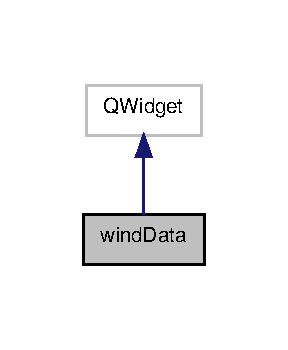
\includegraphics[width=138pt]{classwind_data__inherit__graph}
\end{center}
\end{figure}


Collaboration diagram for wind\+Data\+:\nopagebreak
\begin{figure}[H]
\begin{center}
\leavevmode
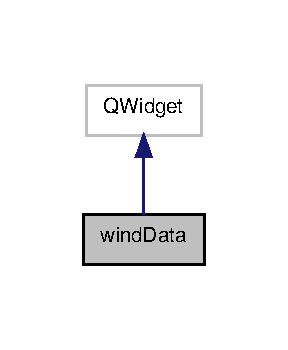
\includegraphics[width=138pt]{classwind_data__coll__graph}
\end{center}
\end{figure}
\subsection*{Public Member Functions}
\begin{DoxyCompactItemize}
\item 
\hyperlink{classwind_data_a90c7b3022b8bf9a59c35b4d8325be4c7}{wind\+Data} (Q\+Widget $\ast$parent=0)
\end{DoxyCompactItemize}


\subsection{Detailed Description}
Widget to collect wind data and plot a time history on the screen 

\subsection{Constructor \& Destructor Documentation}
\hypertarget{classwind_data_a90c7b3022b8bf9a59c35b4d8325be4c7}{\index{wind\+Data@{wind\+Data}!wind\+Data@{wind\+Data}}
\index{wind\+Data@{wind\+Data}!wind\+Data@{wind\+Data}}
\subsubsection[{wind\+Data}]{\setlength{\rightskip}{0pt plus 5cm}wind\+Data\+::wind\+Data (
\begin{DoxyParamCaption}
\item[{Q\+Widget $\ast$}]{parent = {\ttfamily 0}}
\end{DoxyParamCaption}
)}}\label{classwind_data_a90c7b3022b8bf9a59c35b4d8325be4c7}


The documentation for this class was generated from the following files\+:\begin{DoxyCompactItemize}
\item 
\hyperlink{wind_data_8h}{wind\+Data.\+h}\item 
\hyperlink{wind_data_8cpp}{wind\+Data.\+cpp}\end{DoxyCompactItemize}

\chapter{File Documentation}
\hypertarget{sample_network_8cpp}{\section{sample\+Network.\+cpp File Reference}
\label{sample_network_8cpp}\index{sample\+Network.\+cpp@{sample\+Network.\+cpp}}
}
{\ttfamily \#include \char`\"{}sample\+Network.\+h\char`\"{}}\\*
Include dependency graph for sample\+Network.\+cpp\+:
\nopagebreak
\begin{figure}[H]
\begin{center}
\leavevmode
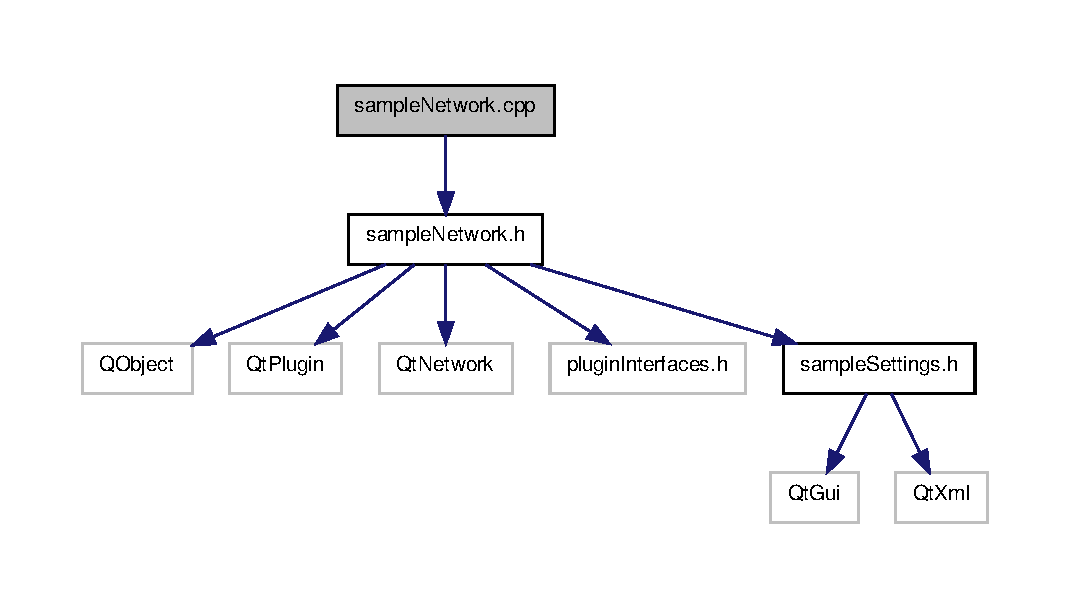
\includegraphics[width=350pt]{sample_network_8cpp__incl}
\end{center}
\end{figure}
\subsection*{Functions}
\begin{DoxyCompactItemize}
\item 
\hyperlink{sample_network_8cpp_a20120930e05d5fc35961b60605222f1f}{Q\+\_\+\+E\+X\+P\+O\+R\+T\+\_\+\+P\+L\+U\+G\+I\+N2} (\hyperlink{classsample_network}{sample\+Network}, \hyperlink{classsample_network}{sample\+Network})
\end{DoxyCompactItemize}


\subsection{Function Documentation}
\hypertarget{sample_network_8cpp_a20120930e05d5fc35961b60605222f1f}{\index{sample\+Network.\+cpp@{sample\+Network.\+cpp}!Q\+\_\+\+E\+X\+P\+O\+R\+T\+\_\+\+P\+L\+U\+G\+I\+N2@{Q\+\_\+\+E\+X\+P\+O\+R\+T\+\_\+\+P\+L\+U\+G\+I\+N2}}
\index{Q\+\_\+\+E\+X\+P\+O\+R\+T\+\_\+\+P\+L\+U\+G\+I\+N2@{Q\+\_\+\+E\+X\+P\+O\+R\+T\+\_\+\+P\+L\+U\+G\+I\+N2}!sample\+Network.\+cpp@{sample\+Network.\+cpp}}
\subsubsection[{Q\+\_\+\+E\+X\+P\+O\+R\+T\+\_\+\+P\+L\+U\+G\+I\+N2}]{\setlength{\rightskip}{0pt plus 5cm}Q\+\_\+\+E\+X\+P\+O\+R\+T\+\_\+\+P\+L\+U\+G\+I\+N2 (
\begin{DoxyParamCaption}
\item[{{\bf sample\+Network}}]{, }
\item[{{\bf sample\+Network}}]{}
\end{DoxyParamCaption}
)}}\label{sample_network_8cpp_a20120930e05d5fc35961b60605222f1f}

\hypertarget{sample_network_8h}{\section{sample\+Network.\+h File Reference}
\label{sample_network_8h}\index{sample\+Network.\+h@{sample\+Network.\+h}}
}
{\ttfamily \#include $<$Q\+Object$>$}\\*
{\ttfamily \#include $<$Qt\+Plugin$>$}\\*
{\ttfamily \#include $<$Qt\+Network$>$}\\*
{\ttfamily \#include $<$plugin\+Interfaces.\+h$>$}\\*
{\ttfamily \#include \char`\"{}sample\+Settings.\+h\char`\"{}}\\*
Include dependency graph for sample\+Network.\+h\+:
\nopagebreak
\begin{figure}[H]
\begin{center}
\leavevmode
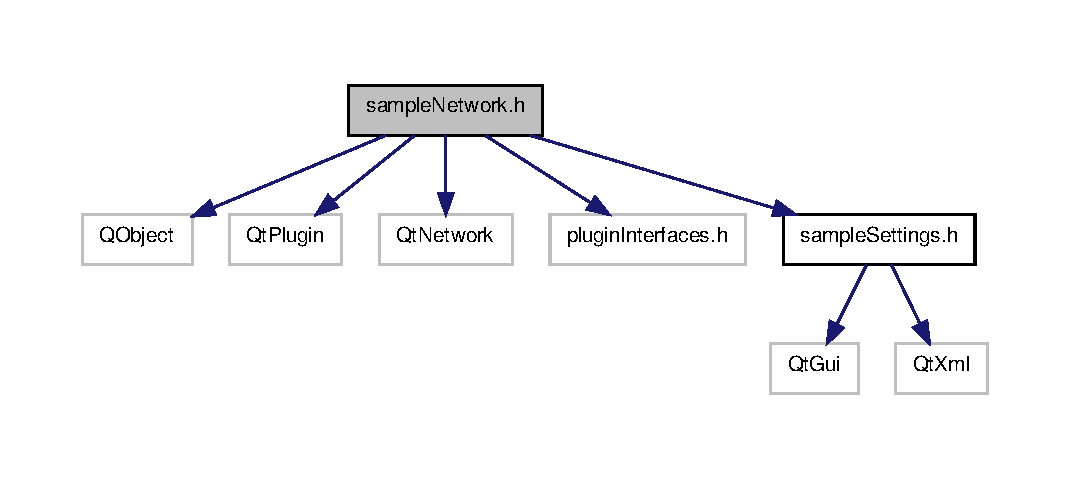
\includegraphics[width=350pt]{sample_network_8h__incl}
\end{center}
\end{figure}
This graph shows which files directly or indirectly include this file\+:\nopagebreak
\begin{figure}[H]
\begin{center}
\leavevmode
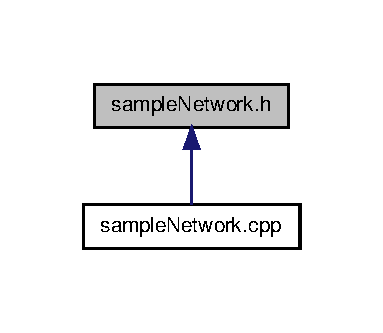
\includegraphics[width=184pt]{sample_network_8h__dep__incl}
\end{center}
\end{figure}
\subsection*{Classes}
\begin{DoxyCompactItemize}
\item 
class \hyperlink{classsample_network}{sample\+Network}
\end{DoxyCompactItemize}

\hypertarget{sample_settings_8cpp}{\section{sample\+Settings.\+cpp File Reference}
\label{sample_settings_8cpp}\index{sample\+Settings.\+cpp@{sample\+Settings.\+cpp}}
}
{\ttfamily \#include $<$Qt\+Gui$>$}\\*
{\ttfamily \#include $<$Qt\+Xml$>$}\\*
{\ttfamily \#include $<$math.\+h$>$}\\*
{\ttfamily \#include \char`\"{}sample\+Settings.\+h\char`\"{}}\\*
Include dependency graph for sample\+Settings.\+cpp\+:\nopagebreak
\begin{figure}[H]
\begin{center}
\leavevmode
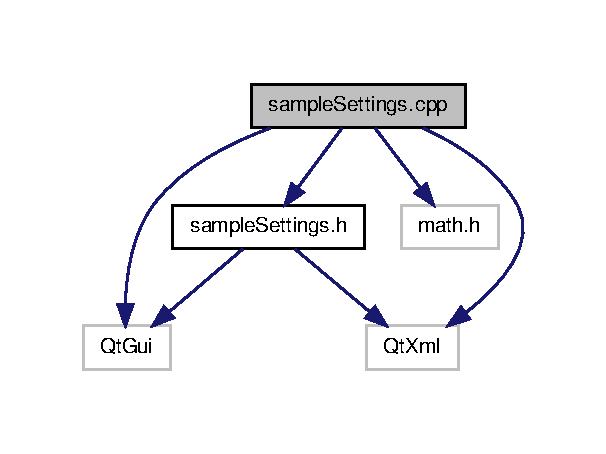
\includegraphics[width=291pt]{sample_settings_8cpp__incl}
\end{center}
\end{figure}

\hypertarget{sample_settings_8h}{\section{sample\+Settings.\+h File Reference}
\label{sample_settings_8h}\index{sample\+Settings.\+h@{sample\+Settings.\+h}}
}
{\ttfamily \#include $<$Qt\+Gui$>$}\\*
{\ttfamily \#include $<$Qt\+Xml$>$}\\*
Include dependency graph for sample\+Settings.\+h\+:\nopagebreak
\begin{figure}[H]
\begin{center}
\leavevmode
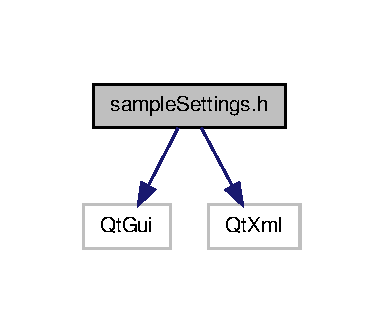
\includegraphics[width=184pt]{sample_settings_8h__incl}
\end{center}
\end{figure}
This graph shows which files directly or indirectly include this file\+:\nopagebreak
\begin{figure}[H]
\begin{center}
\leavevmode
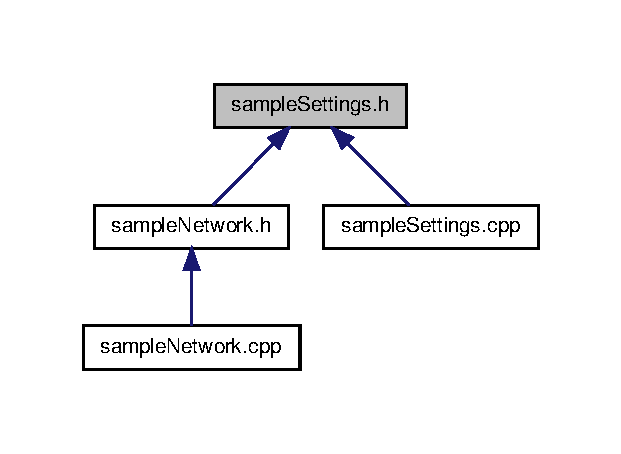
\includegraphics[width=298pt]{sample_settings_8h__dep__incl}
\end{center}
\end{figure}
\subsection*{Classes}
\begin{DoxyCompactItemize}
\item 
class \hyperlink{classsample_settings}{sample\+Settings}
\end{DoxyCompactItemize}

\hypertarget{wind_data_8cpp}{\section{wind\+Data.\+cpp File Reference}
\label{wind_data_8cpp}\index{wind\+Data.\+cpp@{wind\+Data.\+cpp}}
}
{\ttfamily \#include \char`\"{}wind\+Data.\+h\char`\"{}}\\*
Include dependency graph for wind\+Data.\+cpp\+:\nopagebreak
\begin{figure}[H]
\begin{center}
\leavevmode
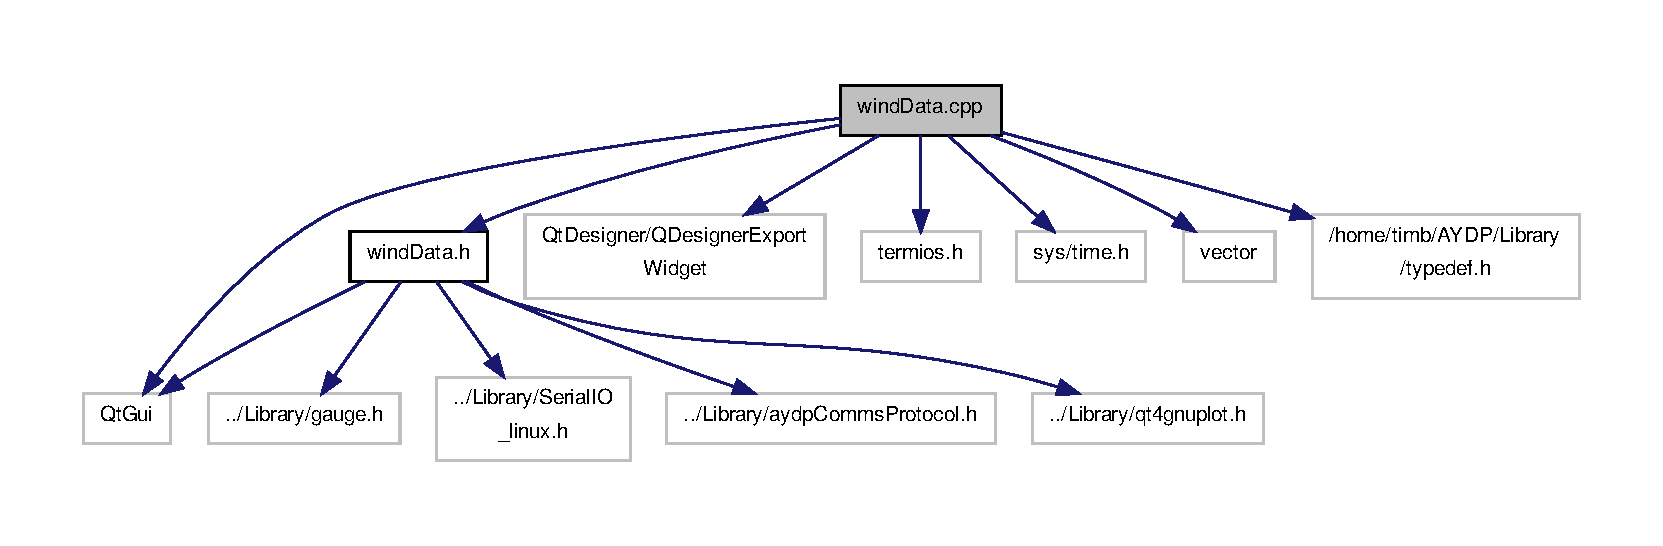
\includegraphics[width=350pt]{wind_data_8cpp__incl}
\end{center}
\end{figure}

\hypertarget{wind_data_8h}{\section{wind\+Data.\+h File Reference}
\label{wind_data_8h}\index{wind\+Data.\+h@{wind\+Data.\+h}}
}
{\ttfamily \#include $<$Qt\+Gui$>$}\\*
{\ttfamily \#include \char`\"{}../\+Library/gauge.\+h\char`\"{}}\\*
{\ttfamily \#include \char`\"{}../\+Library/\+Serial\+I\+O\+\_\+linux.\+h\char`\"{}}\\*
{\ttfamily \#include \char`\"{}../\+Library/aydp\+Comms\+Protocol.\+h\char`\"{}}\\*
{\ttfamily \#include \char`\"{}../\+Library/qt4gnuplot.\+h\char`\"{}}\\*
Include dependency graph for wind\+Data.\+h\+:\nopagebreak
\begin{figure}[H]
\begin{center}
\leavevmode
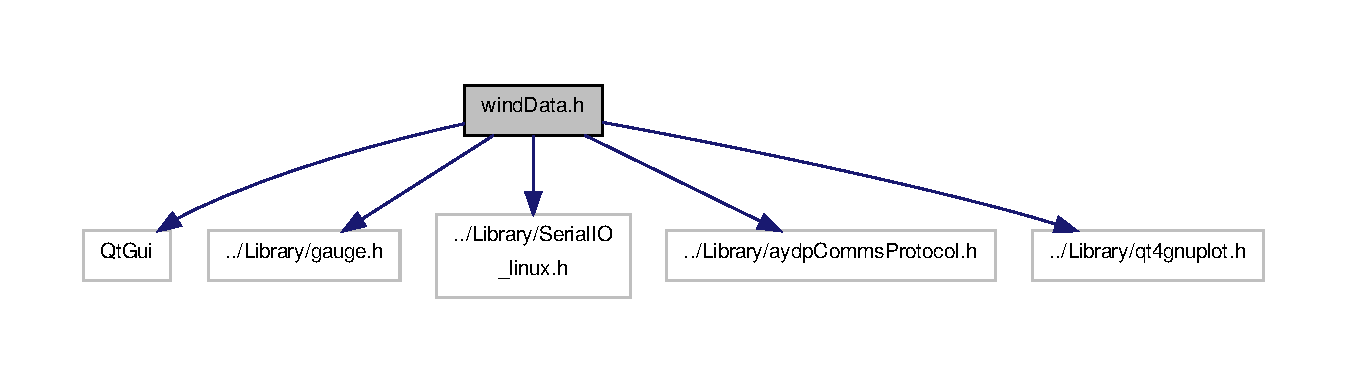
\includegraphics[width=350pt]{wind_data_8h__incl}
\end{center}
\end{figure}
This graph shows which files directly or indirectly include this file\+:\nopagebreak
\begin{figure}[H]
\begin{center}
\leavevmode
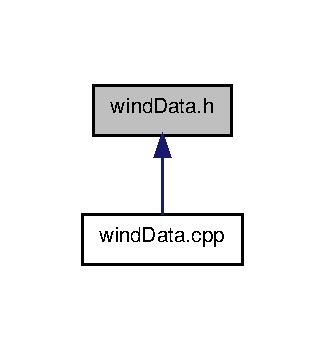
\includegraphics[width=156pt]{wind_data_8h__dep__incl}
\end{center}
\end{figure}
\subsection*{Classes}
\begin{DoxyCompactItemize}
\item 
class \hyperlink{classwind_data}{wind\+Data}
\end{DoxyCompactItemize}

%--- End generated contents ---

% Index
\newpage
\phantomsection
\addcontentsline{toc}{chapter}{Index}
\printindex

\end{document}
